\subsection{Method definition}

This method is inspired by ``fake-rate'' methods~\cite{fakeLeptonNote1,fakeLeptonNote2}, in which the efficiency to pass a tight numerator cut with respect to a looser denominator cut is measured in a control sample enriched in background.  This fake-rate is then applied to the background dominated denominator and not numerator selection in the signal sample.  In the \zm~method, the difference between the denominator and numerator is the cut on the MET.  We first evaluate the efficiency to pass the signal MET cut given a loose denominator cut in a photon+jets control sample, and then apply this efficiency to the \dyll dominated dilepton events that pass the denominator cut and fail the numerator cut in the dilepton sample. 
The estimate of the residual \dyll background in the dilepton sample can be expressed more formally as:

\begin{equation}
N_B\left(\mathrm{pass}\right)=N_B\left(\mathrm{fail}\right) \cdot \zm~,
\end{equation}

Where $N_B\left(\mathrm{pass}\right)$ is the number of \dyll background events after the signal \met~ cut and
$N_B\left(\mathrm{fail}\right)$ is the number of \dyll background events that fail the signal \met~ cut but pass the 
loose denominator cut.  The \met~ fake rate, $\zm~$, is the efficiency to pass the signal \met~ cut 
given the loose denominator cut has passed as measured in the independent \gjets~control sample.  

The \gjets~ control sample can also be used to extract alternate shapes for variables
that can defined consistently on both this sample and the dilepton sample.  
The alternate shapes can be extracted by weighting the \gjets~ sample on an event by event
basis according to \zm.  This is analogous to the derivation of kinematic shapes
for the \Wjets~ background \cite{ref:shapenote}, as used in the 2011 Higgs analysis.

The method is valid if the fake \met~ spectrum, in \gjets~events models the fake \met spectrum in \dyll events well.
Because the main source of fake \met~ in both the \dyll and \gjets~samples is the mis-measurement 
of the hadronic recoil and pileup effects, this is a reasonable starting assumption.

To take into account the kinematic differences between the \dyll and \gjets~samples, \zm
is defined in bins of jet multiplicity ($N_{jets}$) and photon transverse momentum ($p_{T}\left(\gamma\right)$)
as follows:

\begin{equation}
\zeta\left(N_{jets},p_{T}\left(\gamma\right)\right)=\frac{N\left(N_{jets},p_{T}\left(\gamma\right), \met>\mwp\right)}{N\left(N_{jets},p_{T}\left(\gamma\right),\met<\mwp\right)}
\end{equation}

where $\mwp$ represents the working point chosen for the final \met~cut in the analyis.
In the same flavor dilepton sample, events passing the final analysis
selection but with $\met<\mwp$ are selected and \zm~is used to extrapolate to the signal region:

\begin{equation}
N_{\dyll}\left(\met>\mwp,N_{jets},p_{T}\left(\dil\right)\right)= \zeta\left(N_{jets},p_{T}\left(\dil\right)\right) \cdot N_{\dyll}\left(\met<\mwp,N_{jets},p_{T}\left(\dil\right)\right)
\end{equation}

where, in data, $N_{\dyll}\left(\met<\mwp\right)$ is computed subtracting opposite flavor and \V\Z~ events.

\subsection{The \hww~case}

In the \hww~analysis we consider events with dilepton $p_T$$>$45 \GeVc~and $\mathrm{min}$-$\mathrm{pmet}$$>$20 \GeV~ as a baseline common to same and opposite flavor final state~\cite{ref:hwwsmurfs};

$\mathrm{min}$-$\mathrm{pmet}$ is defined as:
\begin{equation}
\text{min-pmet} = \text{min(proj-pfMet,proj-trackMet)} ,
\end{equation}

where ``pfMet'' is the \met~reconstructed with the particle flow algorithm, ``trackMet'' is the \met~ constructed from charged particles consistent 
with originating from the primary vertex.
The ``proj-met'' variable (where met is either pfMet or trackMet) is defined as:

\begin{equation}
\text{proj-met} = 
\begin{cases} \met & \text{if $\Delta\phi_{min}>\frac{\pi}{2}$,}
\\
\met\sin(\Delta\phi_{min}) & \text{if $\Delta\phi_{min}<\frac{\pi}{2}$}
\end{cases}
\end{equation}
\begin{equation}
\text{with } \Delta\phi_{min} =  min(\Delta\phi(\ell_1,\met),\Delta\phi(\ell_2,\met))\\
\end{equation}
where $\Delta\phi(\ell_i,\met)$ is the angle between \met\ and lepton $i$ in the transverse plane;
the main purpose for using ``proj-met'' is to reduce the impact of lepton mismeasurement.
It also acts to further suppress the contribution from \dytt.
The final \met~ selection in the same flavor dilepton final state requires min-pmet$>$(37+nvtx/2) \GeV. 

In the photon sample this selection is reproduced by cutting on min-met=$\mathrm{min(pfMet,trackMet)}$ and photon $p_T$.
In photon events, ``proj-met'' variables cannot be defined because is not possible to project on lepton directions, so the \zm~ method will not 
predict the contribution from fake \met~due to lepton mismesurement. 
However, as it shown in Figures \ref{fig:met_0j}-\ref{fig:met_1j}, despite the slightly different definiton, the photon sample reproduces with 
good precision the \met in the \dyll~sample.

Is summary, we use the following definitions:
\begin{itemize}
\item dilepton sample pass region: min-pmet$>$(37+nvtx/2) \GeV, dilepton $p_T$$>$45 \GeVc
\item dilepton sample fail region: 20$<$min-pmet$<$(37+nvtx/2) \GeV, dilepton $p_T$$>$45 \GeVc
\item photon sample pass region: min-met$>$(37+nvtx/2) \GeV, photon $p_T$$>$45 \GeVc
\item photon sample fail region: 20$<$min-met$<$(37+nvtx/2) \GeV, photon $p_T$$>$45 \GeVc
\end{itemize}

%%%%%%%%
\begin{figure}[!hbtp]
\begin{center}
\subfigure[proj-pfMet in \dyll~ sample]{\label{subfig:pmet_0j}
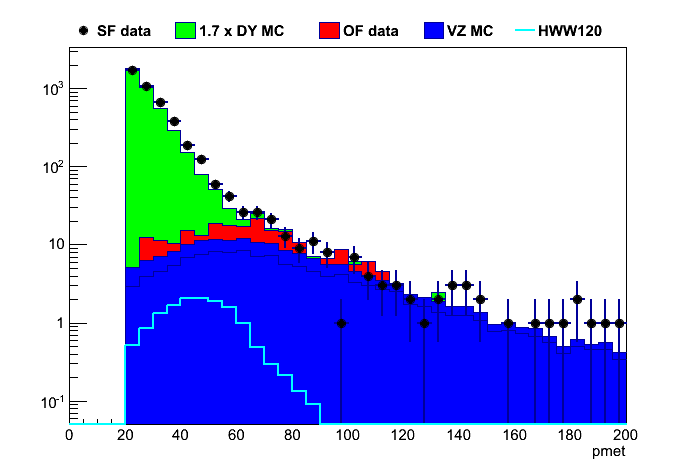
\includegraphics[width=.4\textwidth]{figures/pmet_0j.png}}
\subfigure[pfMet in \gjets~ sample]{\label{subfig:met_0j}
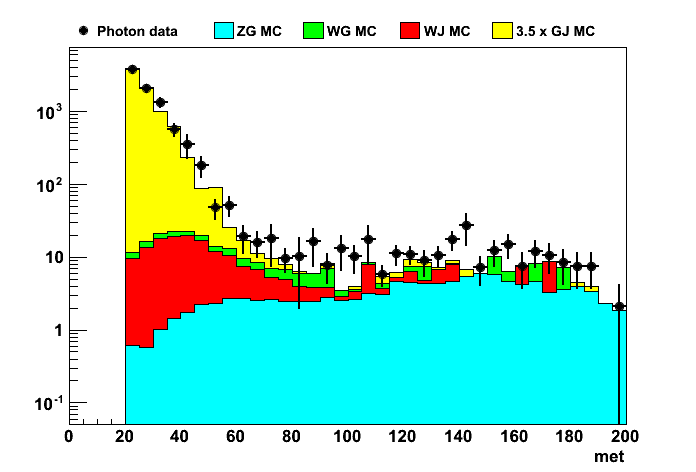
\includegraphics[width=.4\textwidth]{figures/met_0j.png}}\\
\subfigure[proj-trackMet in \dyll~ sample]{\label{subfig:pTrackMet_0j}
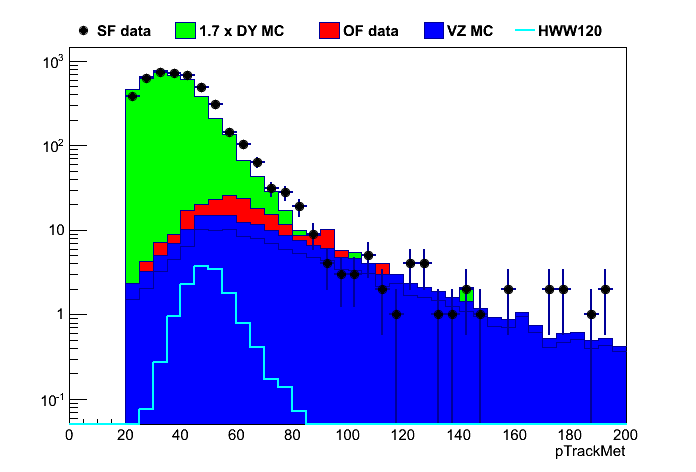
\includegraphics[width=.4\textwidth]{figures/pTrackMet_0j.png}}
\subfigure[trackMet in \gjets~ sample]{\label{subfig:trackMet_0j}
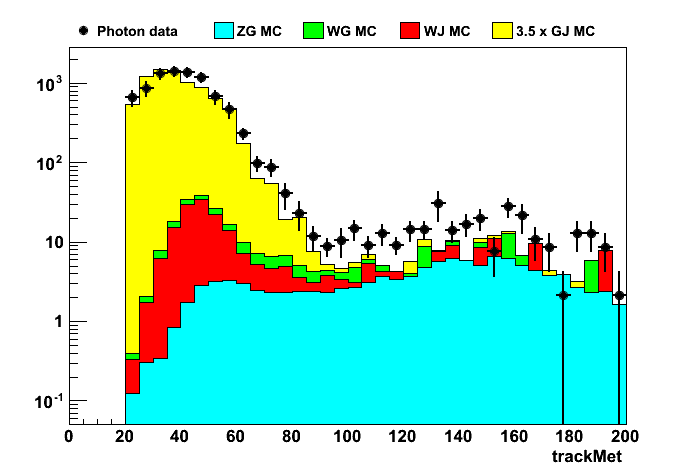
\includegraphics[width=.4\textwidth]{figures/trackMet_0j.png}}
\caption{\met in the 0-jet bin. 
For visualization purposes, the \gjets~ and \dyll~contributions from MC are scaled by a had-hoc scale factor to macth data in the bulk of the distribution.
In the \gjets~ sample, data is shown after re-weighting to the \dyll~$p_T$ distribution in MC events.}
\label{fig:met_0j}
\end{center}
\end{figure}
%%%%%%%%

%%%%%%%%
\begin{figure}[!hbtp]
\begin{center}
\subfigure[proj-pfMet in \dyll~ sample]{\label{subfig:pmet_1j}
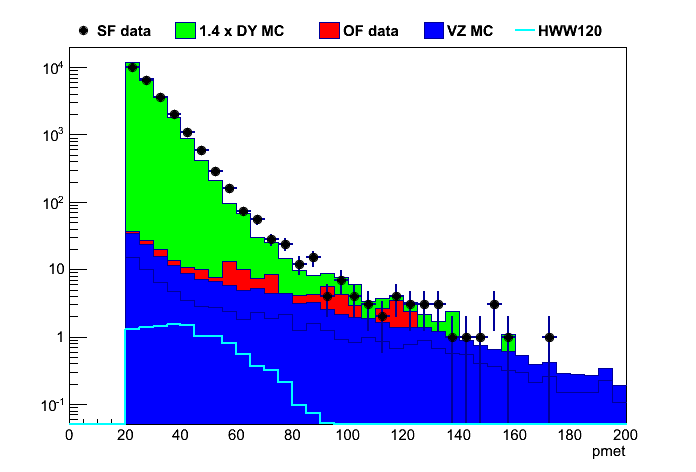
\includegraphics[width=.4\textwidth]{figures/pmet_1j.png}}
\subfigure[pfMet in \gjets~ sample]{\label{subfig:met_1j}
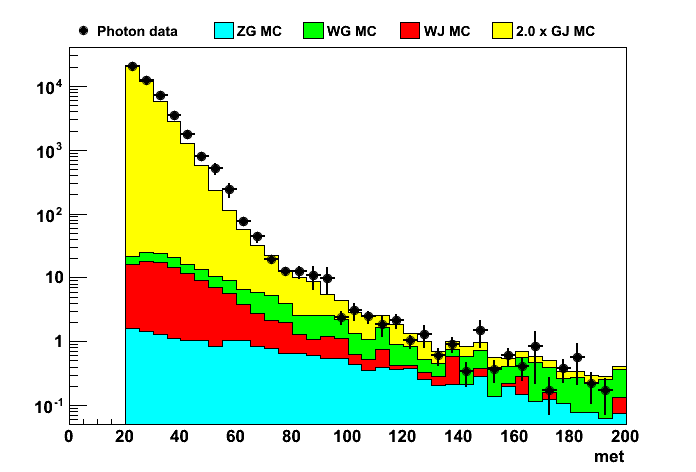
\includegraphics[width=.4\textwidth]{figures/met_1j.png}}\\
\subfigure[proj-trackMet in \dyll~ sample]{\label{subfig:pTrackMet_1j}
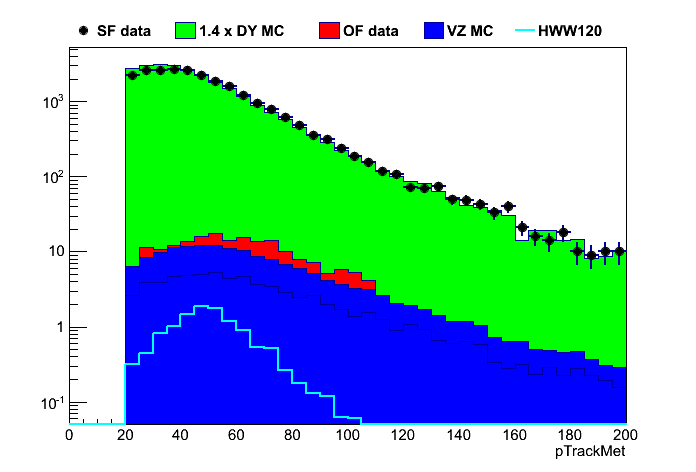
\includegraphics[width=.4\textwidth]{figures/pTrackMet_1j.png}}
\subfigure[trackMet in \gjets~ sample]{\label{subfig:trackMet_1j}
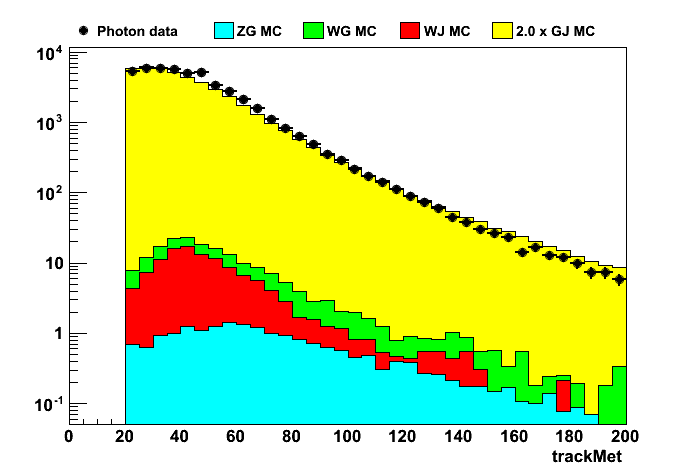
\includegraphics[width=.4\textwidth]{figures/trackMet_1j.png}}
\caption{\met in the 1-jet bin. 
For visualization purposes, the \gjets~ and \dyll~contributions from MC are scaled by a had-hoc scale factor to macth data in the bulk of the distribution.
In the \gjets~ sample, data is shown after re-weighting to the \dyll~$p_T$ distribution in MC events.}
\label{fig:met_1j}
\end{center}
\end{figure}
%%%%%%%%

%%%%%%%%
\begin{figure}[!hbtp]
\begin{center}
\subfigure[proj-pfMet in \dyll~ sample]{\label{subfig:pmet_2j}
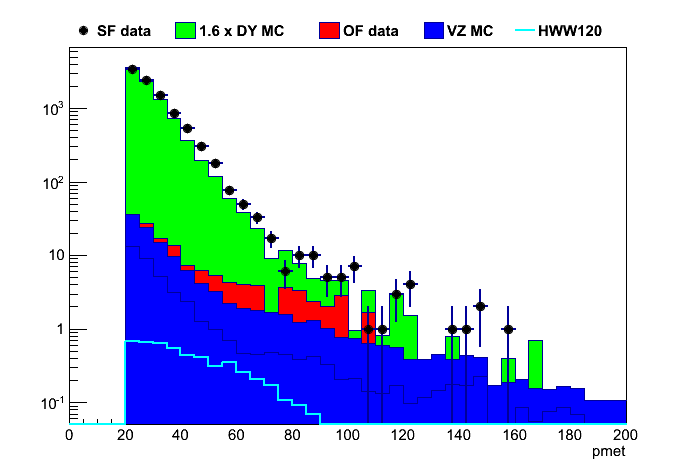
\includegraphics[width=.4\textwidth]{figures/pmet_2j.png}}
\subfigure[pfMet in \gjets~ sample]{\label{subfig:met_2j}
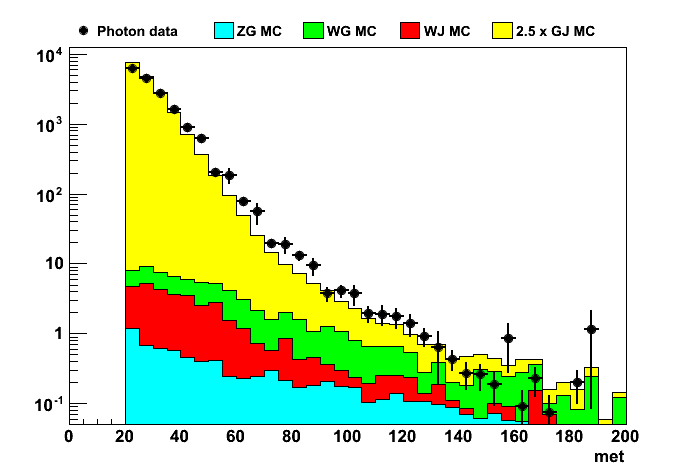
\includegraphics[width=.4\textwidth]{figures/met_2j.png}}\\
\subfigure[proj-trackMet in \dyll~ sample]{\label{subfig:pTrackMet_2j}
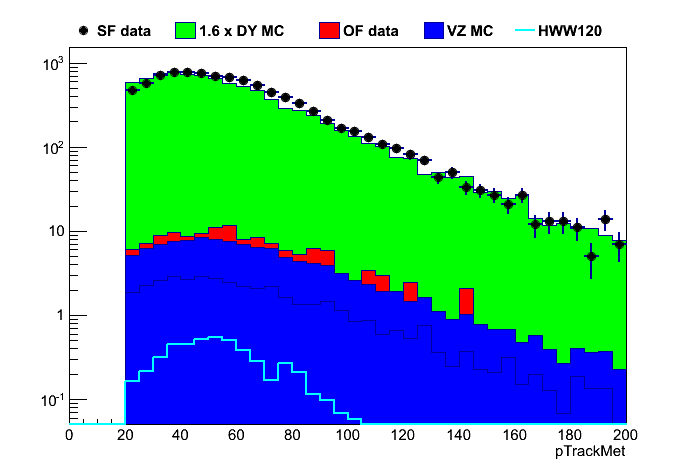
\includegraphics[width=.4\textwidth]{figures/pTrackMet_2j.png}}
\subfigure[trackMet in \gjets~ sample]{\label{subfig:trackMet_2j}
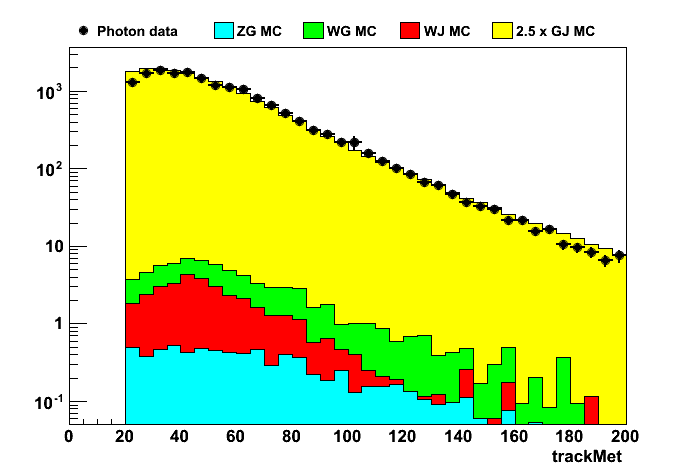
\includegraphics[width=.4\textwidth]{figures/trackMet_2j.png}}
\caption{\met in the 2-jet bin. 
For visualization purposes, the \gjets~ and \dyll~contributions from MC are scaled by a had-hoc scale factor to macth data in the bulk of the distribution.
In the \gjets~ sample, data is shown after re-weighting to the \dyll~$p_T$ distribution in MC events.}
\label{fig:met_2j}
\end{center}
\end{figure}
%%%%%%%%

\clearpage

\subsection{Evaluation of \zm}

For each jet bin, \zm~ is evaluated both on MC and data samples in bins of photon $p_T$.
In data, the expected backgrounds with non-fake \met~ are subtracted from the photon sample.
Results for WW level in  are shown in Figures~\ref{fig:zeta_MC} and~\ref{fig:zeta_mh0}.
These are the values used for the \hww~ BDT shape analysis.

In the cut based analysis, an additional narrow cut on the transverse Higgs mass is applied~\cite{ref:hwwsmurfs}, where the following definition of $m_T$ is used:
\begin{equation}
m_{T} = \sqrt{2\pt^{ll}\met(1-cos(\Delta\phi_{\ell\ell-\met}))}
\end{equation}
where $\Delta\phi_{\ell\ell-\met}$ is the angle between dilepton direction and \met\ in the transverse plane.
For example, in the \mHi=120 \GeVcc~ analysis the signal region requires 70$<$$m_T$$<$120 \GeVcc.
Given that \met\ and $m_T$ are correlated variables, the \zm\ value depends on the $m_T$ cut value; 
therefore, \zm\ is derived separately for each Higgs mass analysis applying the corresponding $m_T$ cut on the photon sample.

A few representative results for \zm~derived from data for Higgs level cut based analysis are shown in Figures~\ref{fig:zeta_mh120}-\ref{fig:zeta_mh160}.

%%%%%%%%
\begin{figure}[!hbtp]
\begin{center}
\subfigure[0-jet]{\label{subfig:zeta_MC_0j_minmet}
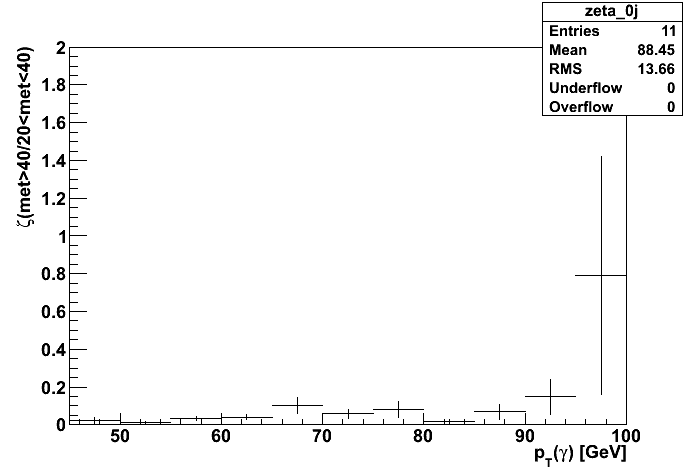
\includegraphics[width=.4\textwidth]{figures/zeta_MC_0j_minmet.png}}
\subfigure[1-jet]{\label{subfig:zeta_MC_1j_minmet}
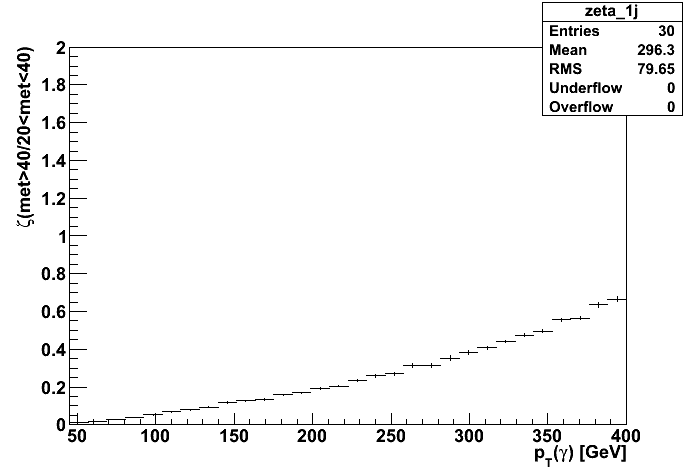
\includegraphics[width=.4\textwidth]{figures/zeta_MC_1j_minmet.png}}\\
\subfigure[2-jet]{\label{subfig:zeta_MC_2j_minmet}
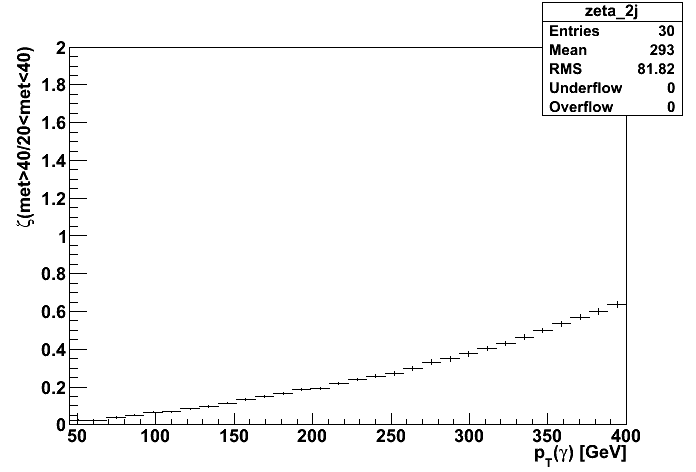
\includegraphics[width=.4\textwidth]{figures/zeta_MC_2j_minmet.png}}
\caption{\zm~in MC at \WW~level.}
\label{fig:zeta_MC}
\end{center}
\end{figure}
%%%%%%%%

%%%%%%%%
\begin{figure}[!hbtp]
\begin{center}
\subfigure[0-jet]{\label{subfig:zeta_mass0_0j_minmet}
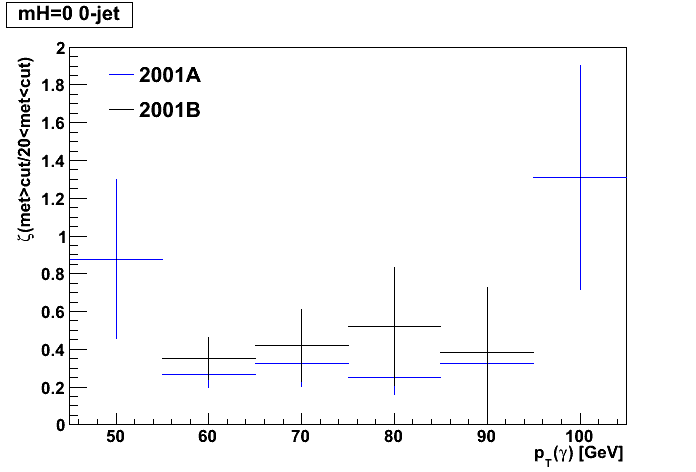
\includegraphics[width=.4\textwidth]{figures/zeta_mass0_0j_minmet.png}}
\subfigure[1-jet]{\label{subfig:zeta_mass0_1j_minmet}
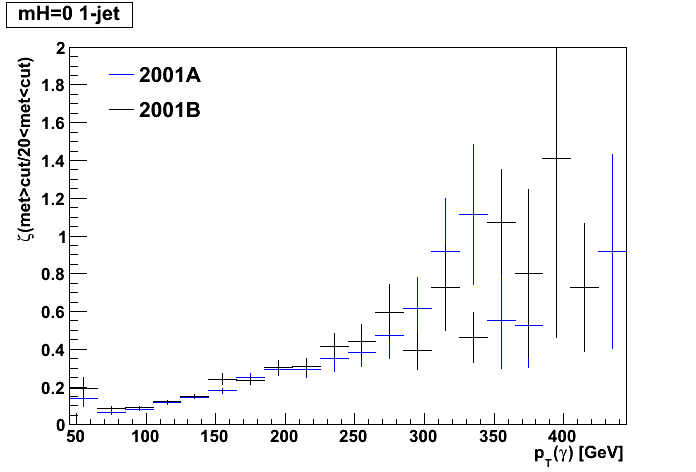
\includegraphics[width=.4\textwidth]{figures/zeta_mass0_1j_minmet.png}}\\
\subfigure[2-jet]{\label{subfig:zeta_mass0_2j_minmet}
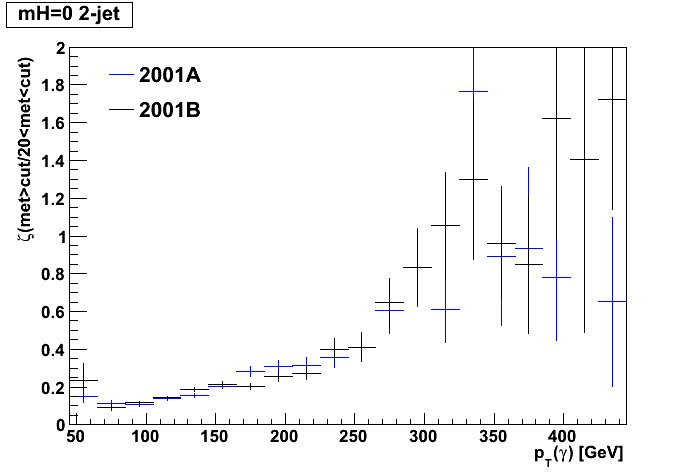
\includegraphics[width=.4\textwidth]{figures/zeta_mass0_2j_minmet.png}}
\caption{\zm~in data at \WW~level.}
\label{fig:zeta_mh0}
\end{center}
\end{figure}
%%%%%%%%

%%%%%%%%
\begin{figure}[!hbtp]
\begin{center}
\subfigure[0-jet]{\label{subfig:zeta_mass120_0j_minmet}
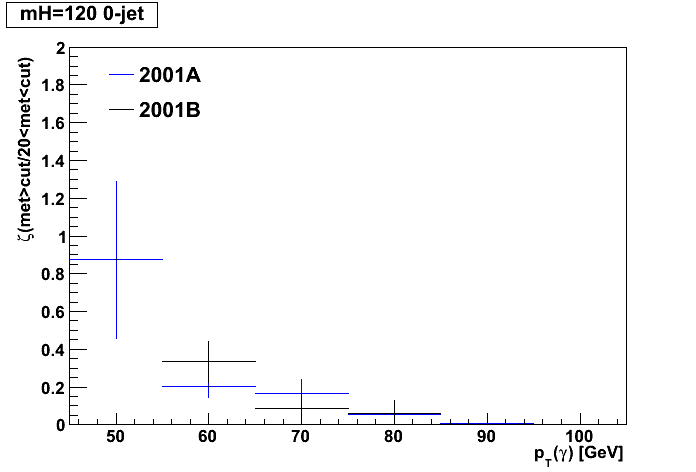
\includegraphics[width=.4\textwidth]{figures/zeta_mass120_0j_minmet.png}}
\subfigure[1-jet]{\label{subfig:zeta_mass120_1j_minmet}
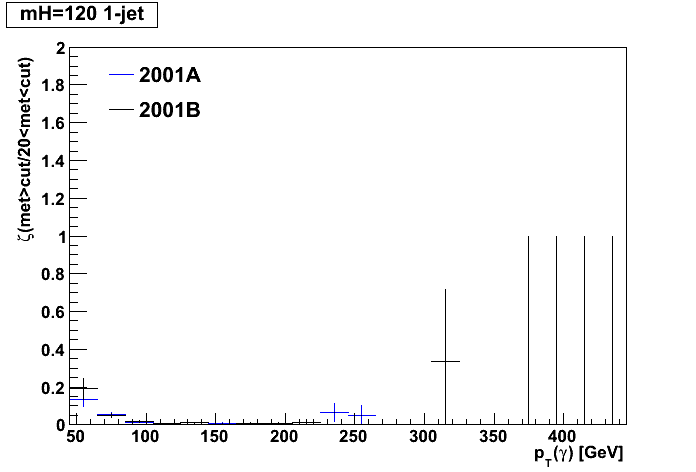
\includegraphics[width=.4\textwidth]{figures/zeta_mass120_1j_minmet.png}}\\
\subfigure[2-jet]{\label{subfig:zeta_mass120_2j_minmet}
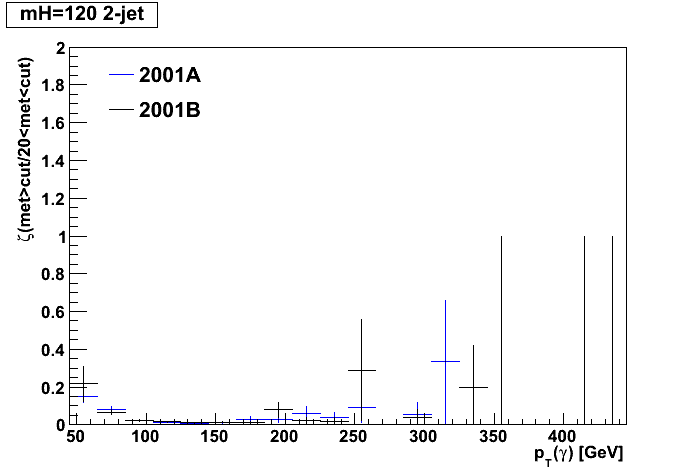
\includegraphics[width=.4\textwidth]{figures/zeta_mass120_2j_minmet.png}}
\caption{\zm~in data for \mHi=120 \GeVcc.}
\label{fig:zeta_mh120}
\end{center}
\end{figure}
%%%%%%%%

%%%%%%%%
\begin{figure}[!hbtp]
\begin{center}
\subfigure[0-jet]{\label{subfig:zeta_mass140_0j_minmet}
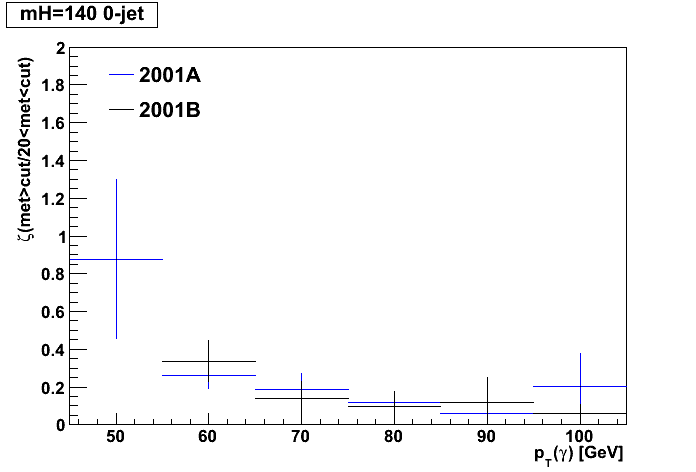
\includegraphics[width=.4\textwidth]{figures/zeta_mass140_0j_minmet.png}}
\subfigure[1-jet]{\label{subfig:zeta_mass140_1j_minmet}
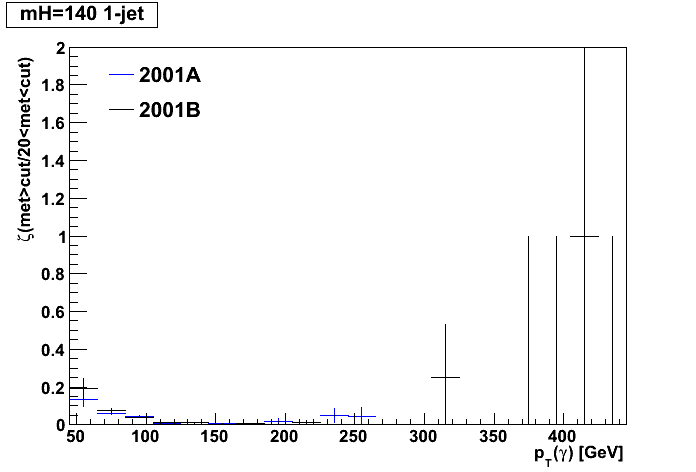
\includegraphics[width=.4\textwidth]{figures/zeta_mass140_1j_minmet.png}}\\
\subfigure[2-jet]{\label{subfig:zeta_mass140_2j_minmet}
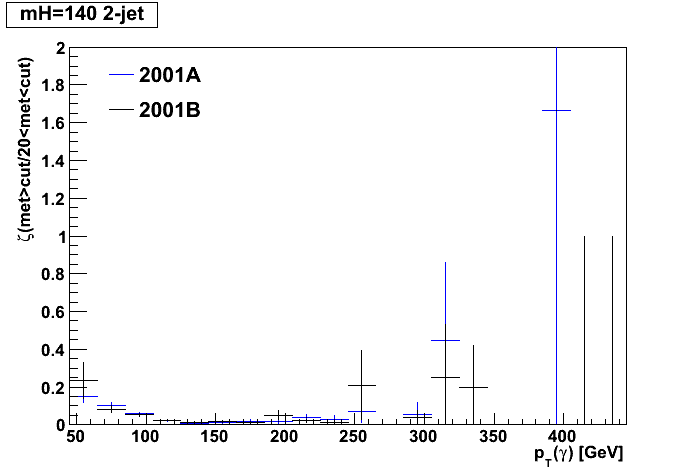
\includegraphics[width=.4\textwidth]{figures/zeta_mass140_2j_minmet.png}}
\caption{\zm~in data for \mHi=140 \GeVcc.}
\label{fig:zeta_mh140}
\end{center}
\end{figure}
%%%%%%%%

%%%%%%%%
\begin{figure}[!hbtp]
\begin{center}
\subfigure[0-jet]{\label{subfig:zeta_mass160_0j_minmet}
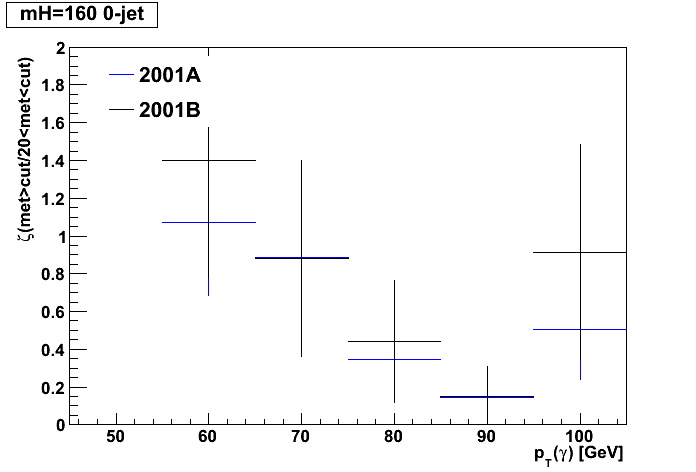
\includegraphics[width=.4\textwidth]{figures/zeta_mass160_0j_minmet.png}}
\subfigure[1-jet]{\label{subfig:zeta_mass160_1j_minmet}
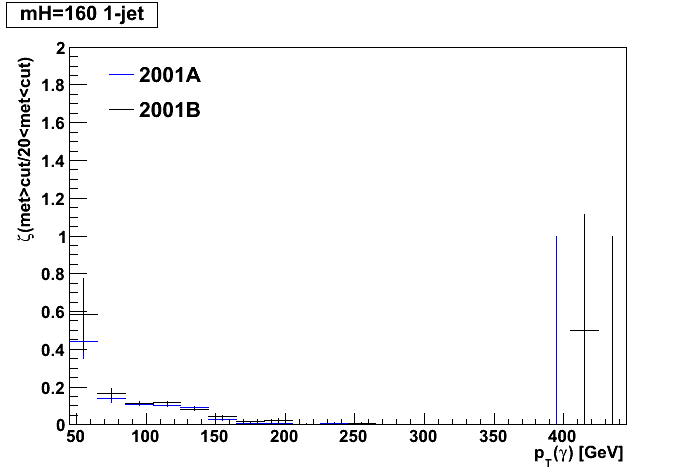
\includegraphics[width=.4\textwidth]{figures/zeta_mass160_1j_minmet.png}}\\
\subfigure[2-jet]{\label{subfig:zeta_mass160_2j_minmet}
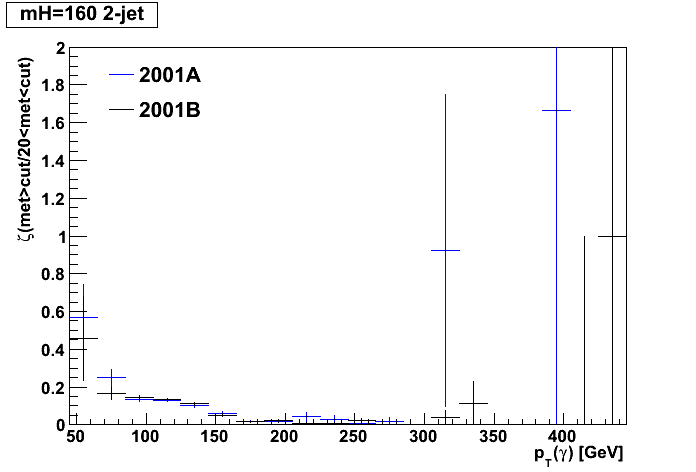
\includegraphics[width=.4\textwidth]{figures/zeta_mass160_2j_minmet.png}}
\caption{\zm~in data for \mHi=160 \GeVcc.}
\label{fig:zeta_mh160}
\end{center}
\end{figure}
%%%%%%%%

\clearpage
